% This is samplepaper.tex, a sample chapter demonstrating the
% LLNCS macro package for Springer Computer Science proceedings;
% Version 2.20 of 2017/10/04
%
\documentclass[runningheads]{llncs}
%
\usepackage{graphicx}
\usepackage{float}
\usepackage{hyperref}
% Used for displaying a sample figure. If possible, figure files should
% be included in EPS format.
%
% If you use the hyperref package, please uncomment the following line
% to display URLs in blue roman font according to Springer's eBook style:
% \renewcommand\UrlFont{\color{blue}\rmfamily}

\begin{document}
%
\title{Advanced Data Challenge Seminar\\
		Avito Demand Prediction}
%

% If the paper title is too long for the running head, you can set
% an abbreviated paper title here
%
\author{Simon Giebenhain \and Jonas Probst}
%

% First names are abbreviated in the running head.
% If there are more than two authors, 'et al.' is used.
%
\institute{University of Konstanz\\
\email{simon.giebenhain@uni-konstanz.de}\\
\email{jonas.probst@uni-konstanz.de}}
%
\maketitle              % typeset the header of the contribution
%
\begin{abstract}
This report gives a step-by-step description on how we tackled the Avito\footnote{\url{www.avito.ru}} Demand Prediction Challenge on Kaggle\footnote{\url{www.kaggle.com/c/avito-demand-prediction}} and gives an overview of the used models, one LightGBM and one Neural Network. The goal of the challenge was to predict 'deal probability' (the probability that an ad actually sold something) for an advertisement on Avito based the ads parameters. Python\footnote{\url{www.python.com}} was used as a programming language, with Keras\footnote{\url{www.keras.io}} as an API to work on Neural Networks.

\keywords{Kaggle \and Avito \and Demand Prediction \and Data Challenge}
\end{abstract}
%
%
%
	\section{Data Overview}

\subsection{Dataset}
Avito provided the following files for the challenge, asking the Kaggle community to predict the target variable deal\_probability:
\begin{itemize}
	\item \textbf{train.csv:} Contains approximately 1.5 million training examples, sampled from 15.3.2017 until 28.3.2017.
	\item \textbf{test.csv:} Contains approximately 500 000 test examples, sampled from 12.4.2017 until 18.4.2017.
	\item \textbf{train\_active and test\_active:} Supplemental Data from ads that were displayed in the same time periods, but not contained in the train or test dataset. Does not include images or deal\_probability.
	\item \textbf{periods\_train and periods\_test:} Supplemental data showing the dates when the ads from train\_active and test\_active were activated and displayed.
	\item \textbf{train\_jpg.zip and test\_jpg.zip:} Images from ads in train.csv and test.csv.
	\item \textbf{sample\_submission.csv:} A sample submission in the correct format.\\
	\begin{center}
	\begin{tabular}{|c|c|}
		\hline 
		\textbf{item\_id} & \textbf{deal\_probability} \\ 
		\hline 
		1 & 0 \\ 
		\hline 
		4 & 0.1 \\ 
		\hline 
		126 & 0.6 \\ 
		\hline 
		... & ... \\ 
		\hline 
	\end{tabular} 
	\end{center} 
\end{itemize}

\subsection{Data Schema}  

Each data sample in train.csv and test.csv corresponds to one advertisement. The features are described in the following table. \\

\begin{table}
\begin{tabular}{|c|c|c|}
	\hline 
	\textbf{Name} & \textbf{Data Type} & \textbf{Description} \\ 
	\hline 
	item\_id & String & Ad ID. \\ 
	\hline 
	user\_id & String & User ID. \\ 
	\hline 
	region & String & Ad region. \\ 
	\hline 
	city & String & Ad city. \\ 
	\hline 
	parent\_category\_name & String & Top level category. \\ 
	\hline 
	category\_name & String & More fine grained category. \\ 
	\hline 
	param\_1 & String & Optional; Additional parameter for category. \\ 
	\hline 
	param\_2 & String & Optional; Additional parameter for category. \\ 
	\hline 
	param\_3 & String & Optional; Additional parameter for category. \\ 
	\hline 
	title & String & Ad title. \\ 
	\hline 
	description & String & Ad description. \\ 
	\hline 
	price & Float & Ad price. \\ 
	\hline 
	item\_seq\_number & Integer & Ad seqential number for user. \\ 
	\hline 
	activation\_date & Date & Date ad was placed. \\ 
	\hline 
	user\_type & String & User type (Private, Company or Shop) \\ 
	\hline 
	image & String & ID of image. Same as filename. \\ 
	\hline 
	image\_top\_1 & Float & Mystery classification code for image. \\ 
	\hline 
	deal\_probability & Float & \begin{tabular}[c]{@{}c@{}}Target variable.\\ The likelihood that an ad actually sold something. \\No information on how it got calculated.\end{tabular} \\ 
	\hline 
\end{tabular} \\

\caption{Data Schema}
\end{table}

\section{Data Preprocessing}
\subsubsection{Categorical Features:} This section will be discussed with each of our models, because our models require specific preprocessing for categorical variables.
\subsubsection{Numerical Features:}
Because you can sell anything from clothes to houses on Avito, "price" has a huge range, so we normalized it logarithmically.\\
The other numerical features did not need to be preprocessed.
\subsubsection{Activaton Date:} 
We extracted the weekday from "activation\_date" as a number from 0 to 6 and just kept that number. The information about month and "day of month" was not useful, because they did not overlap in the train and test set.

\subsubsection{Missing Values}
 For most columns there are no missing values, because they are mandatory to fill in for uploading an ad or get filled in automatically. "param\_2" and "param\_3" have about 50\% missing values, because they are optional or don't exist for some categories. The description was empty in about 8\%. We filled all these missing values with the empty string, as there is no good way to approximate these values and it may not even be desired because having no description is an interesting information itself.\\ \\
 Image and "image\_top\_1" were also missing in about 8\% of ads, which simply were uploaded without image. Here we actually trained a neural network on the description, title and optional parameters for ads with images to predict "image\_top\_1" because it was such an important variable. It was feasible to do so, because "image\_top\_1" is a categorical variable, which can only take on around 3000 different values.\\ \\
 Price is missing for about 5\%  of ads. There could be multiple reasons for that, for example the price could just be written in the description, could be up for debate our could depend on the amount one wants to buy. So we replaced missing values with -1, because setting it to zero would imply that the item was put up for free.
 

\section{Our Models}
\subsection{LightGBM Model}
LightGBM is a gradient boosting model developed by Microsoft which uses decision tree forests to make predictions. It performs well on huge amounts of data while still being relatively fast to train and easily accessible. Because the given dataset is very large LightGBM seemed like a good choice. \\

We started our model with just the basic features that were given in the main data frame. From there we gradually added more features through feature engineering and external data.

\subsubsection{LightGBM Specific Preprocessing for Categorical Variables:}
LightGBM only works on numerical data, so categorical data needs to be encoded. We used target encoding on "region", "city", "parent\_category\_name", "category\_name", "user\_type", "param\_1", "param\_2", "param\_3", "image\_top\_1".\\
Target encoding replaces the original value with the mean of the target variable value of all columns with the same original value. 

\subsubsection{Baseline Model:} For the first model we just used the normalized price and the encoded categorical data, ignoring text and image features and the supplemental data. \\
Test Error: 0.231
\subsubsection{Basic Text Features:} We proceeded with adding basic text features, by extracting number of words, number of characters and number of unique words from description and title. \\
Test Error: 0.230
\subsubsection{TF-IDF:} The next step to get better understanding of the text data was to add Term Frequency - Inverse Document Frequency data, which gives us information about how strongly a document is defined by a specific word or term.\\
We restricted the TF-IDF to 50000 features for description and 50000 features for title. For both we allowed single words as well as 2-grams and 3-grams.\\
Test Error: 0.225\\
\subsubsection{Stemming:} Because in Russian the word endings depend on the grammatical case they are used in we tried to improve the TF-IDF by using stemming to bring all words in their basic form.
Test Error: 0.224
\subsubsection{Image Features:} From the images, we extracted size, blurriness, basic statistical features for color and brightness (mean, standard deviation, mode, min, max) as well as the top 3 predictions of Resnet, Xception, and Inception\_Resnet. Those features did not improve the model a lot, so we concluded that most of the image features were already encoded in "image\_top\_1".\\
Test Error: 0.2237 
\subsubsection{Aggregated Features:} From the supplemental data we were given we computed for each user and category the average online time for items, the average amount of times the same item was put up for sale and the number of items put up.\\
Test Error: 0.2230
\subsubsection{Final Model:} In our final model we used all previous features, because all of them improved the model at least a bit. We then trained with lower learning rate and increased the number of leaves for the trees from 256 to 1024.\\
Test Error: 0.222

\begin{figure}[H]
	\centering
	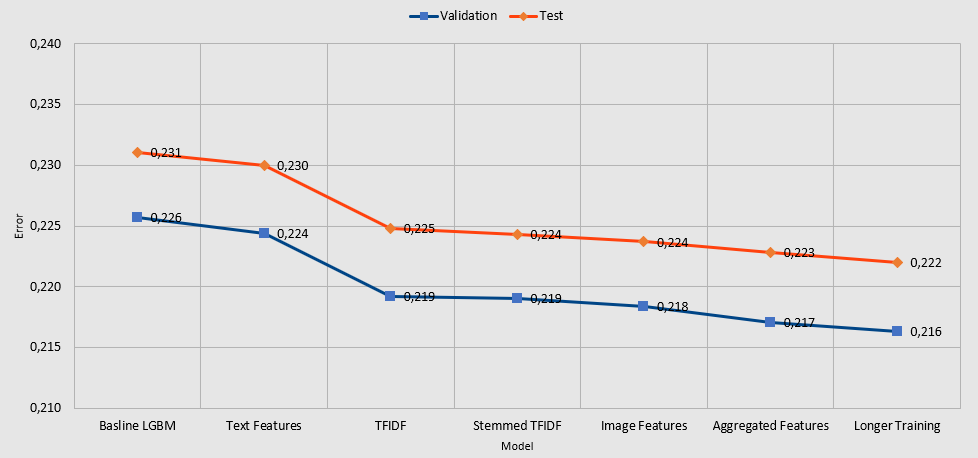
\includegraphics[scale=0.6]{progress}
	\caption[]{Test Error Progress}
	\label{fig:progress}
\end{figure}



\subsection{Neural Network}
 The importance of images in advertisement motivated us, to develop a neural network model, which perform best in high level image analysis tasks. An additional benefit of the neural network model is the potential of a higher level understanding of the text data. In order to make reasonable predictions, the model has to incorporate all different datasets. This led us to develop a  model, which consists of four separate neural networks, one for categorical, one for continuous data one for text and one for image data, combined into a deep and wide neural network.\\
  We fed the network with the same engineered features used for the  LightGBM model, except for the tf-idf data.
  
 \subsubsection{Specific Data Preparation}
 Since neural networks interpret all inputs as numerical variables, one has to carefully preprocess the data, such that there are no false numerical relations in the encoding of the variables. \\
 
 \textit{Numerical Variables:} These variables are already numeric. We tried to normalize the variables to zero mean and unit standard deviation, but this deteriorated the results. Instead we used logarithmic normalization.\\ 
 
 \textit{Categorical Variables:} For each categorical variable we set up a trainable embedding layer of size correlating with the variatey of categories for each variable. \\
 
 \textit{Text:} In order to reduce the computational time and to bring the single text fields into context, we decided to concatenate title, param\_1, param\_2, param\_3 and  description and separate them by a special character. We included the param fields, because sometimes important information is omitted in the title and put into param\_1, param\_2 or param\_3 instead.\\
 Furthermore we did not apply stemming or other preprocessing(e.g. emoji removal), because the neural network should be powerful enough to make use of such information.\\
 In our initial attempts we used word embeddings which were pretrained on russian common crawl. Later on we trained our own word embeddings on the combined text from the train, test, train\_active and test\_active datasets. We used 300 dimensional embeddings, as in the pretrained word embeddings and trained with the CBOW technique.\\
 The performance increased roughly by 0.0008 with the self trained embeddings. Altough this might look like a small improvement, for this challenge this is significant progress.
 
 \textit{Images:} As usual with image analysis using neural networks we downsampled all images, in this case to 299x299 pixels, and normalized the pixels to zero mean and unit standard deviation. Missing images were replaced with images filled with zeros. \\
 
 \subsubsection{Architecture}
The architecture of our deep and wide network is explained by figure \ref{fig:architecture} below.\\
In this figure "FC layer" stands for fully connected layer and is actually an abbreviation for a Dense layer, followed by a Batch Normalization layer, a LeakyReLU activation and Dropout (usually somewhere between 0.2 and 0.5 depending on the size of the layer).
 
\begin{figure}
	\centering
	\includegraphics[scale=0.3]{nn_architecture.png}
	\caption[]{Neural Network Architecture}
	\label{fig:architecture}
\end{figure}

 \subsubsection{Training Procedure}
 For training we split off 33\% of the train dataset as a validation dataset.\\
In order to train the deep and wide network, we first trained the single networks separately on deal probability. To achieve this we added a fully connected layer with a single neuron and sigmoid activation on top of each single network. In this way the single networks extract the most important features, which can be found in the second to last layer, describing the deal probability. Then we loaded and froze the weights of the single networks. At this point we were able to train the final fully connected layer combining the features of the bottom neural networks.\\
A major problem we encountered during training was dealing with images. In total there were roughly 70 GB of images. This made it impossible to do the preprocessing explained above prior to training and store the results in a numpy array. Therefore we had to do the preprocessing on the CPUs while training was executed on the GPU. Unfortunately this required reading the images from a hard drive. Because this was extremely slow, we only trained on epoch on a third of the dataset.\\
Furthermore we used early stopping and reduced the learning rate on plateaus.
 \subsubsection{Results}
 Our first and more simple neural network (not described in this report) had 0.2193 training error, 0.2216 validation error and 0.2259 test error. The more elaborate neural network, as described in this report, had 0.2183 train and 0.2197 validation error without using the images. As can be seen the overfitting in the train dataset was significantly reduced. However when adding the images the test error was 0.228. Either we did a mistake in the training procedure while incorporating the images(because we could only train on one third of the images) or somehow this model is exhibiting strong overfitting between train and test dataset, but not within the train dataset.\\
 In summary our neural network did not improve upon the LightGBM model, as was the case for most other participants of the challenge. Still others made good use of their neural networks while  blending their models, where it is crucial
  to have uncorrelated models.\\
 
 \section{Room for Improvement}
 One great thing about this challenge was the huge effort of the Kaggle community. Although nobody managed to come up with game breaking ideas, there were plenty ideas that gave small improvements. It turned out that engineering many clever features accumulated to a good result. Some ideas of the best scoring solutions are shortly explained next:\\
 \begin{itemize}
 	\item For every category or even tuples or triplets of categories, calculate the average deal\_probability, median price and number of ads.
 	\item Statistics reflecting the daily demand and supply for each category
 	\item Training separate neural networks on the active dataset to predict e.g. price, duration of ad
 \end{itemize}

Furthermore model ensembles were crucial for good scoring solutions. Here it turned out to be important to used uncorrelated models. Therefore it was beneficial to use different kinds of models, e.g a LightGBM a XBG and a Neural Network model. \\

 \section{Conclusion}
At first it seemed like the challenge would provide lot's of interesting, important and diverse data, which should suffice to predict the deal probability relatively well. But even the best team, which had a RMSE of 0.215, did not really "solve" the problem, as their error is still relatively large. In comparison, just predicting the mean deal probability for each category gave an RMSE of 0.249, without using any complicated models. This leads us to believe that the real solution to the problem was not given in the data and relies on many more variables which were not provided.

\end{document}